\documentclass{beamer}
\usepackage{tikz,amsmath,hyperref,graphicx,stackrel,animate,media9}
\usetikzlibrary{positioning,shadows,arrows,shapes,calc}
\newcommand{\argmax}{\operatornamewithlimits{argmax}}
\newcommand{\argmin}{\operatornamewithlimits{argmin}}
\mode<presentation>{\usetheme{Frankfurt}}
\AtBeginSection[]
{
  \begin{frame}<beamer>
    \frametitle{Outline}
    \tableofcontents[currentsection,currentsubsection]
  \end{frame}
}
\title{Lecture 6: Music}
\author{Mark Hasegawa-Johnson}
\date{ECE 401: Signal and Image Analysis, Fall 2020}  
\begin{document}

% Title
\begin{frame}
  \maketitle
\end{frame}

% Title
\begin{frame}
  \tableofcontents
\end{frame}

%%%%%%%%%%%%%%%%%%%%%%%%%%%%%%%%%%%%%%%%%%%%
\section[Review]{Review: Spectrum, Fourier Series, and DFT}
\setcounter{subsection}{1}

\begin{frame}
  \frametitle{Two-sided spectrum}

  The {\bf spectrum} of $x(t)$ is the set of frequencies, and their
  associated phasors,
  \[
  \mbox{Spectrum}\left( x(t) \right) =
  \left\{ (f_{-N},a_{-N}), \ldots, (f_0,a_0), \ldots, (f_N,a_N) \right\}
  \]
  such that
  \[
  x(t) = \sum_{k=-N}^N a_ke^{j2\pi f_kt}
  \]
\end{frame}

\begin{frame}
  \frametitle{Summary}
  \begin{itemize}
  \item {\bf Fourier Analysis}  (finding the spectrum, given the waveform):
    \[
    X_k = \frac{1}{T_0}\int_0^{T_0} x(t)e^{-j2\pi kt/T_0}dt
    \]
  \item {\bf Fourier Synthesis}  (finding the waveform, given the spectrum):
    \[
    x(t) = \sum_{k=-\infty}^\infty X_k e^{j2\pi kt/T_0}
    \]
  \item {\bf DFT Analysis}  (finding the spectrum, given the waveform):
    \[
    X[k] = \sum_{n=0}^{N-1} x[n]e^{-j2\pi kn/N}
    \]
  \item {\bf DFT Synthesis} (finding the waveform, given the spectrum):
    \[
    x[n] = \frac{1}{N}\sum_{k=0}^{N-1} X[k] e^{j2\pi kn/N}
    \]
  \end{itemize}
\end{frame}  

%%%%%%%%%%%%%%%%%%%%%%%%%%%%%%%%%%%%%%%%%%%%
\section[Pitch]{Musical Pitch}
\setcounter{subsection}{1}

\begin{frame}
  \frametitle{Pythagorean Tuning}
  \begin{itemize}
  \item Humans have always known that $f_2=2f_1$ (length of one string
    is twice the length of the other) means they are an octave apart
    (``same note'').
  \item A 3:2 ratio ($f_2=1.5f_1$) is a musical perfect fifth.
  \item Pythagoras is attributed with a system of tuning that created
    an 8-note scale by combining 3:2 and 2:1 ratios (``Pythagorean
    tuning''), used in some places until 1600.
  \end{itemize}
\end{frame}

\begin{frame}
  \frametitle{Equal-Tempered Tuning}

  Equal-tempered tuning divides the octave into twelve equal ratios.
  \begin{itemize}
  \item {\bf Semitones:} the number of semitones, $s$, separating two
    tones $f_2$ and $f_1$ is given by
    \[
    s = 12\log_2\left(\frac{f_2}{f_1}\right)
    \]
  \item {\bf Cents:} the number of cents, $n$, separating two tones
    $f_2$ and $f_1$ is given by
    \[
    n = 1200\log_2\left(\frac{f_2}{f_1}\right)
    \]
  \end{itemize}
\end{frame}

\begin{frame}
  \frametitle{Pythagorean vs. Equal-Tempered Tuning}
  \centerline{\fbox{\href{https://en.wikipedia.org/wiki/Pythagorean_tuning}{Pythagorean, Equal-Tempered, and Just Intonation}}}
\end{frame}

\begin{frame}
  \frametitle{Pythagorean vs. Equal-Tempered Tuning}
  \centerline{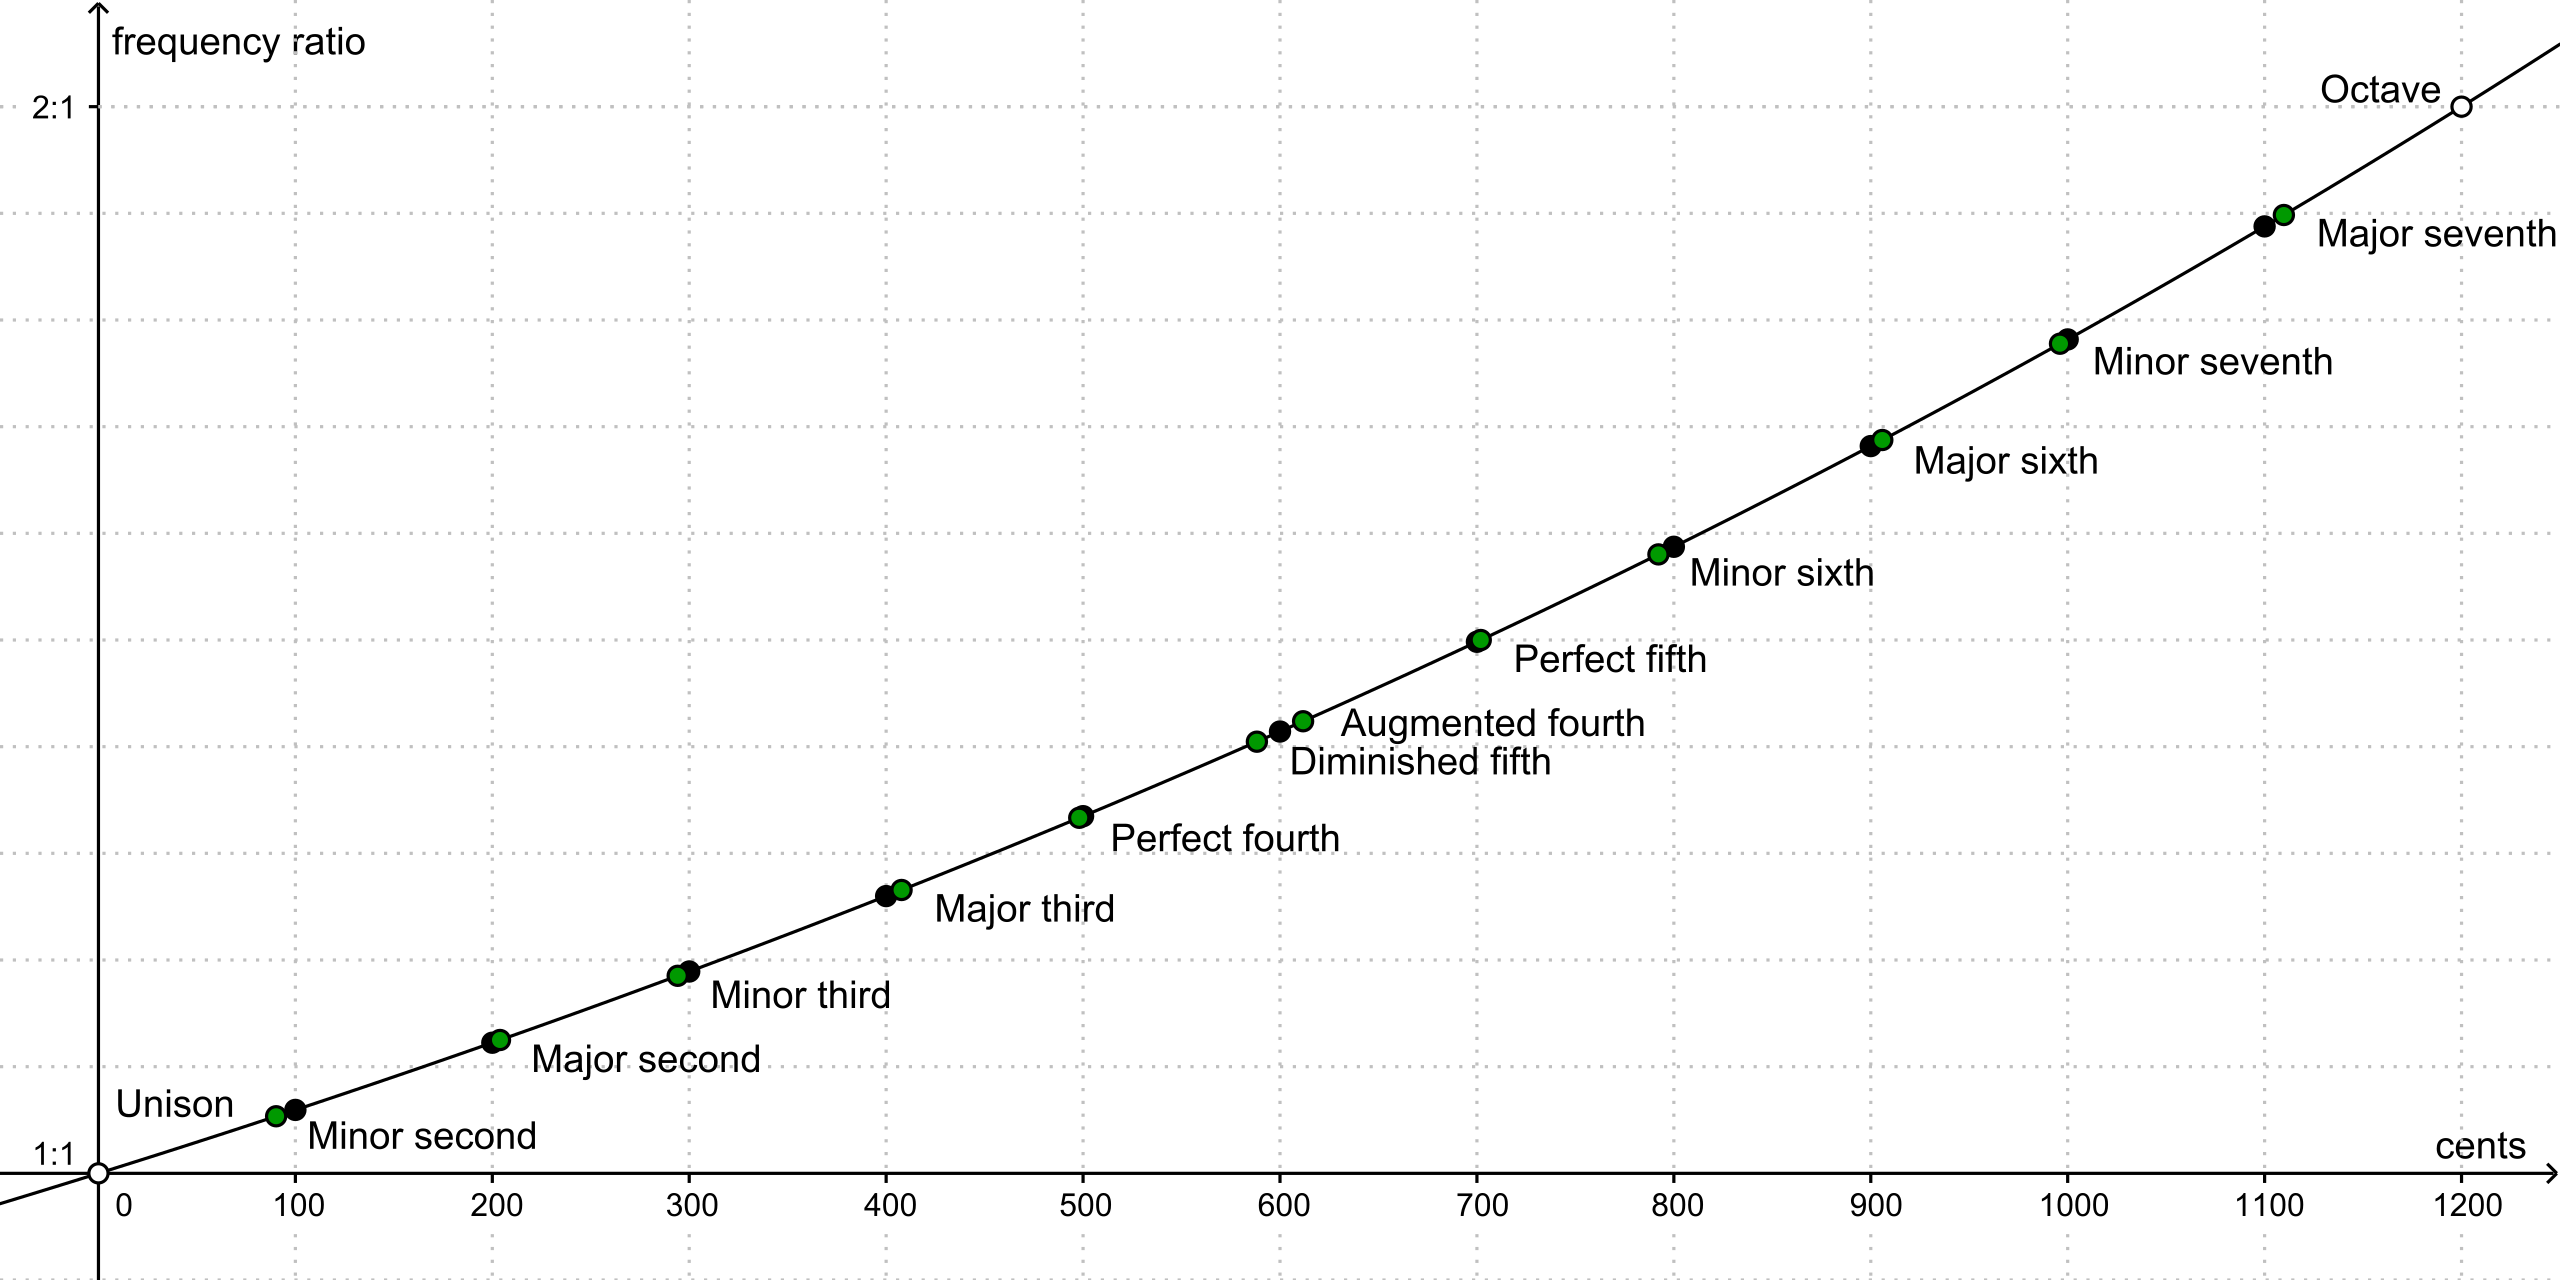
\includegraphics[height=2in]{Music_intervals.png}}
  \begin{tiny}
    By SharkD, public domain image,
    \url{https://commons.wikimedia.org/wiki/File:Music_intervals_frequency_ratio_equal_tempered_pythagorean_comparison.svg}
  \end{tiny}
\end{frame}

%%%%%%%%%%%%%%%%%%%%%%%%%%%%%%%%%%%%%%%%%%%%
\section[Pitch Tracking]{Pitch Tracking: the Harmonic Sieve Algorithm}
\setcounter{subsection}{1}

\begin{frame}
  \frametitle{Pitch Tracking: Intended Output}
  \centerline{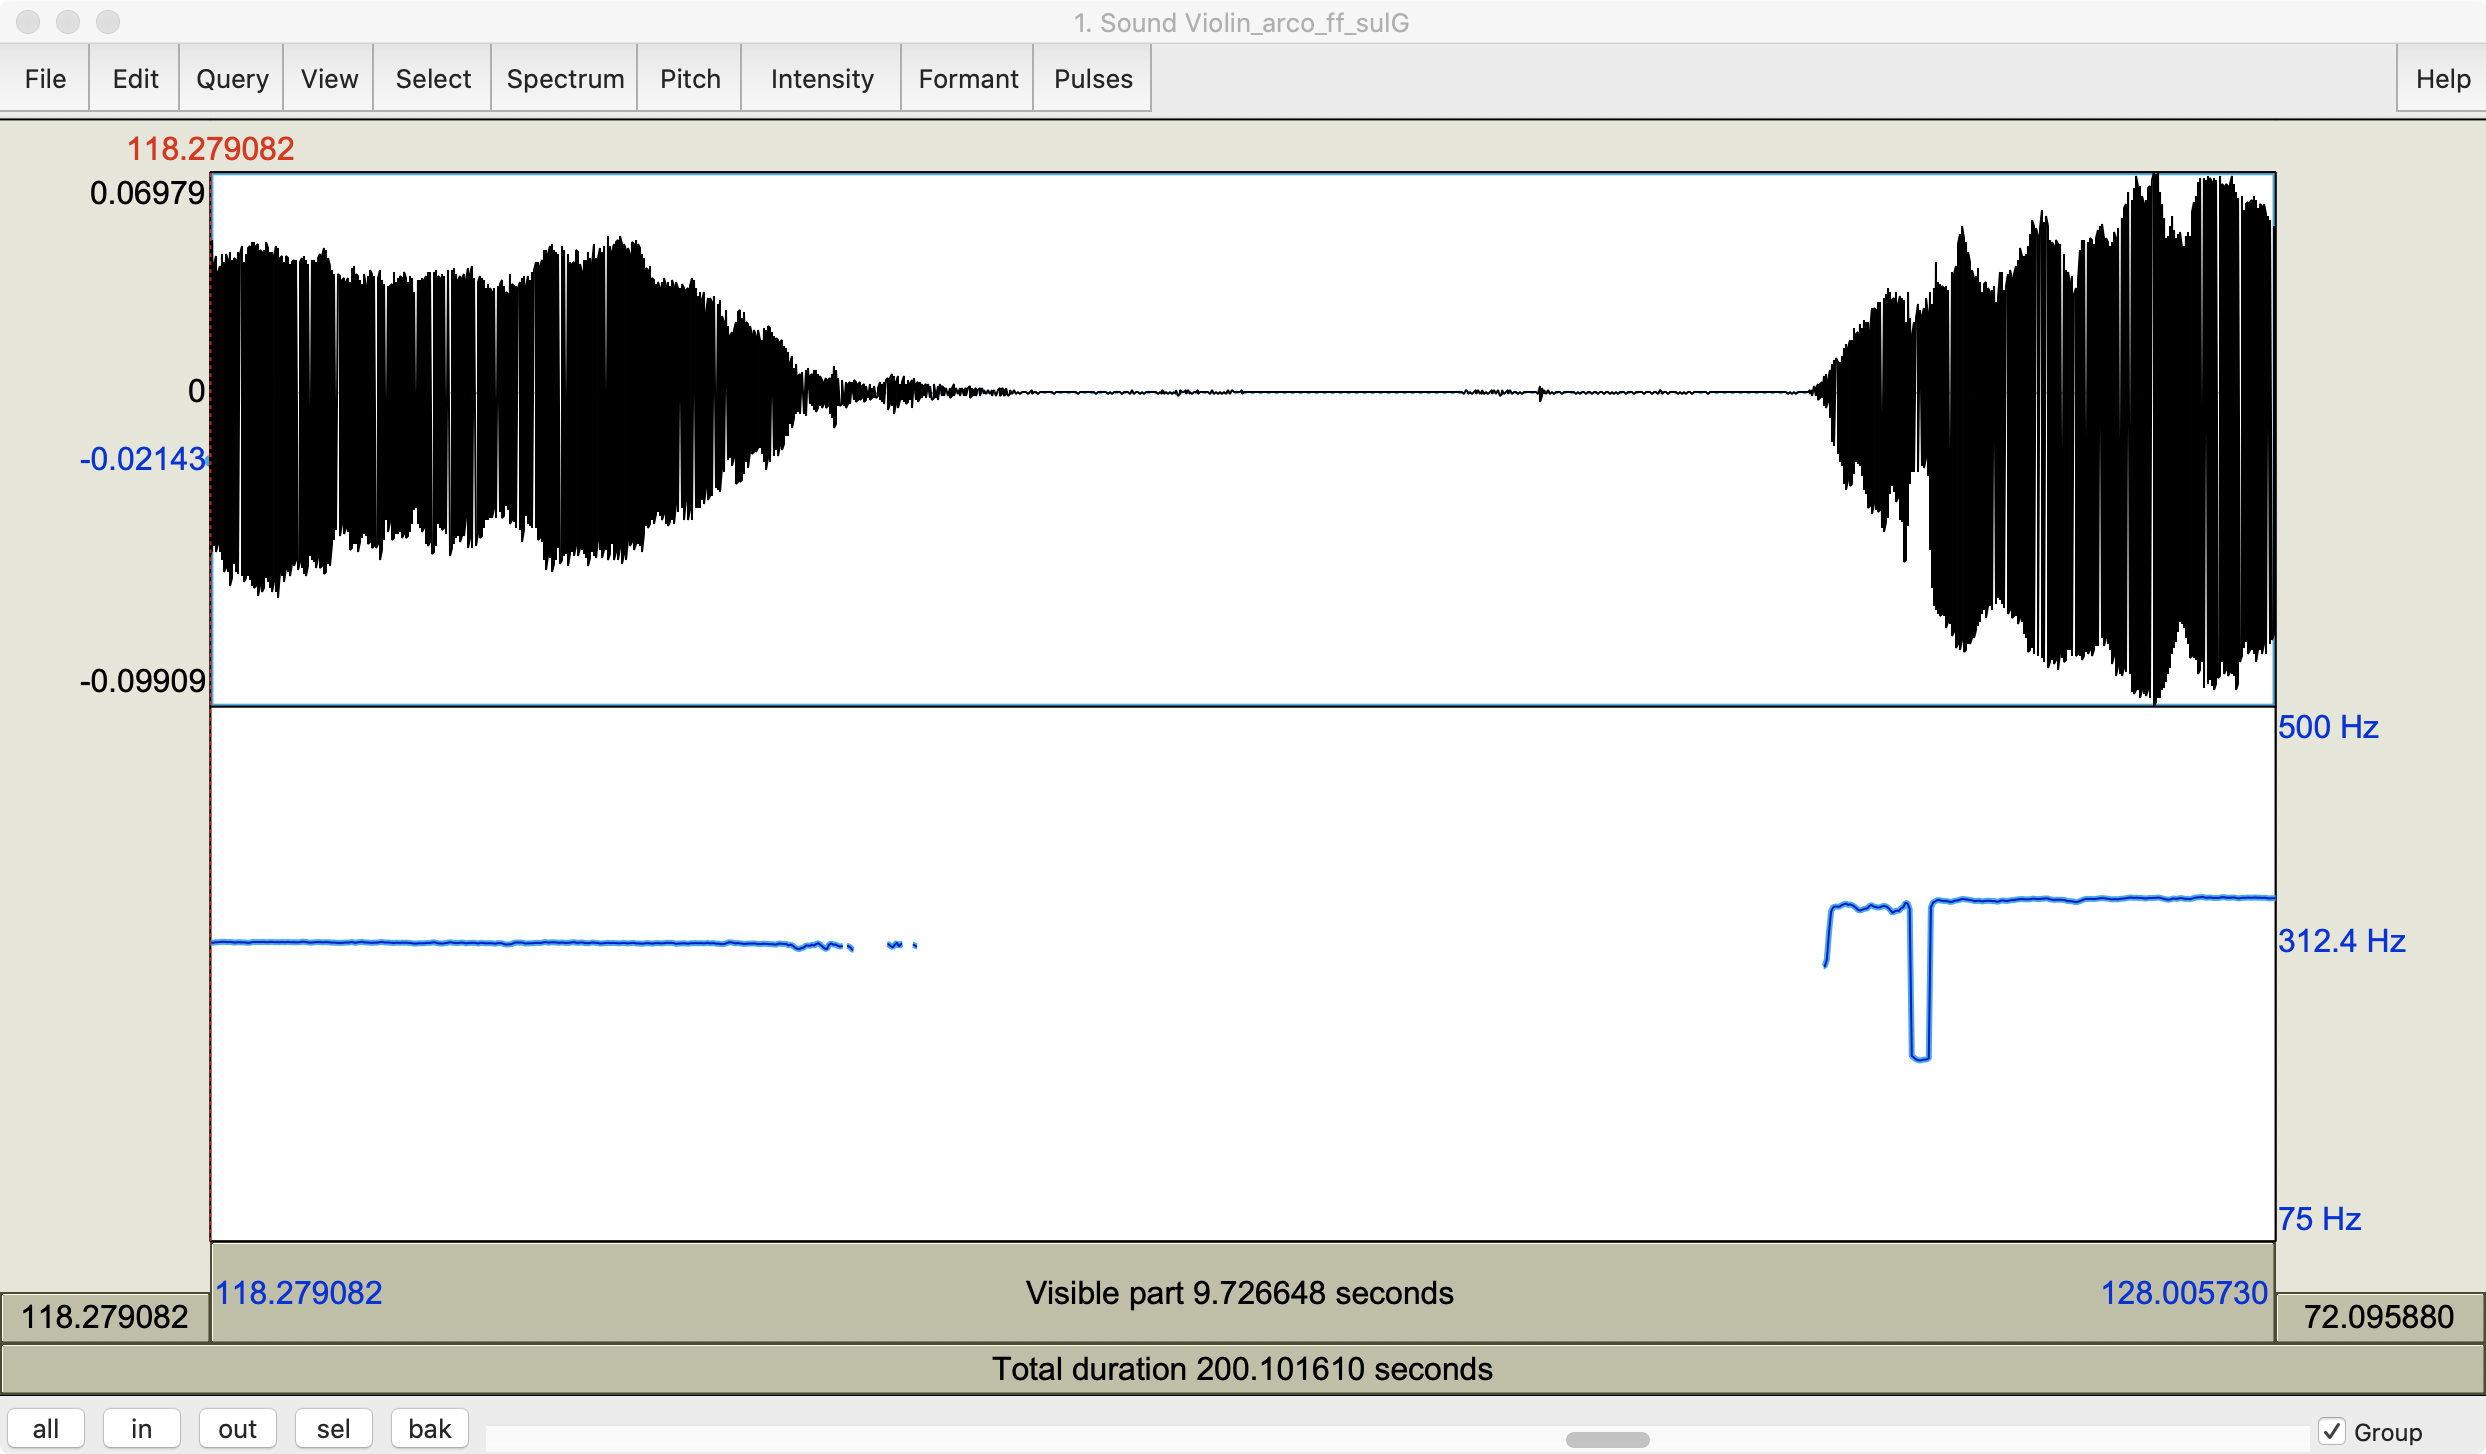
\includegraphics[height=2in]{violin_notes.png}}
\end{frame}

\begin{frame}
  \frametitle{Pitch Tracking: Input}
  \centerline{\fbox{\href{http://theremin.music.uiowa.edu/sound files/MIS/Strings/violin/Violin.arco.ff.sulG.C4Eb5.aiff}{\bf\color{blue}Violin.arco.ff.sulG.C4Eb5.aiff}}}
  \centerline{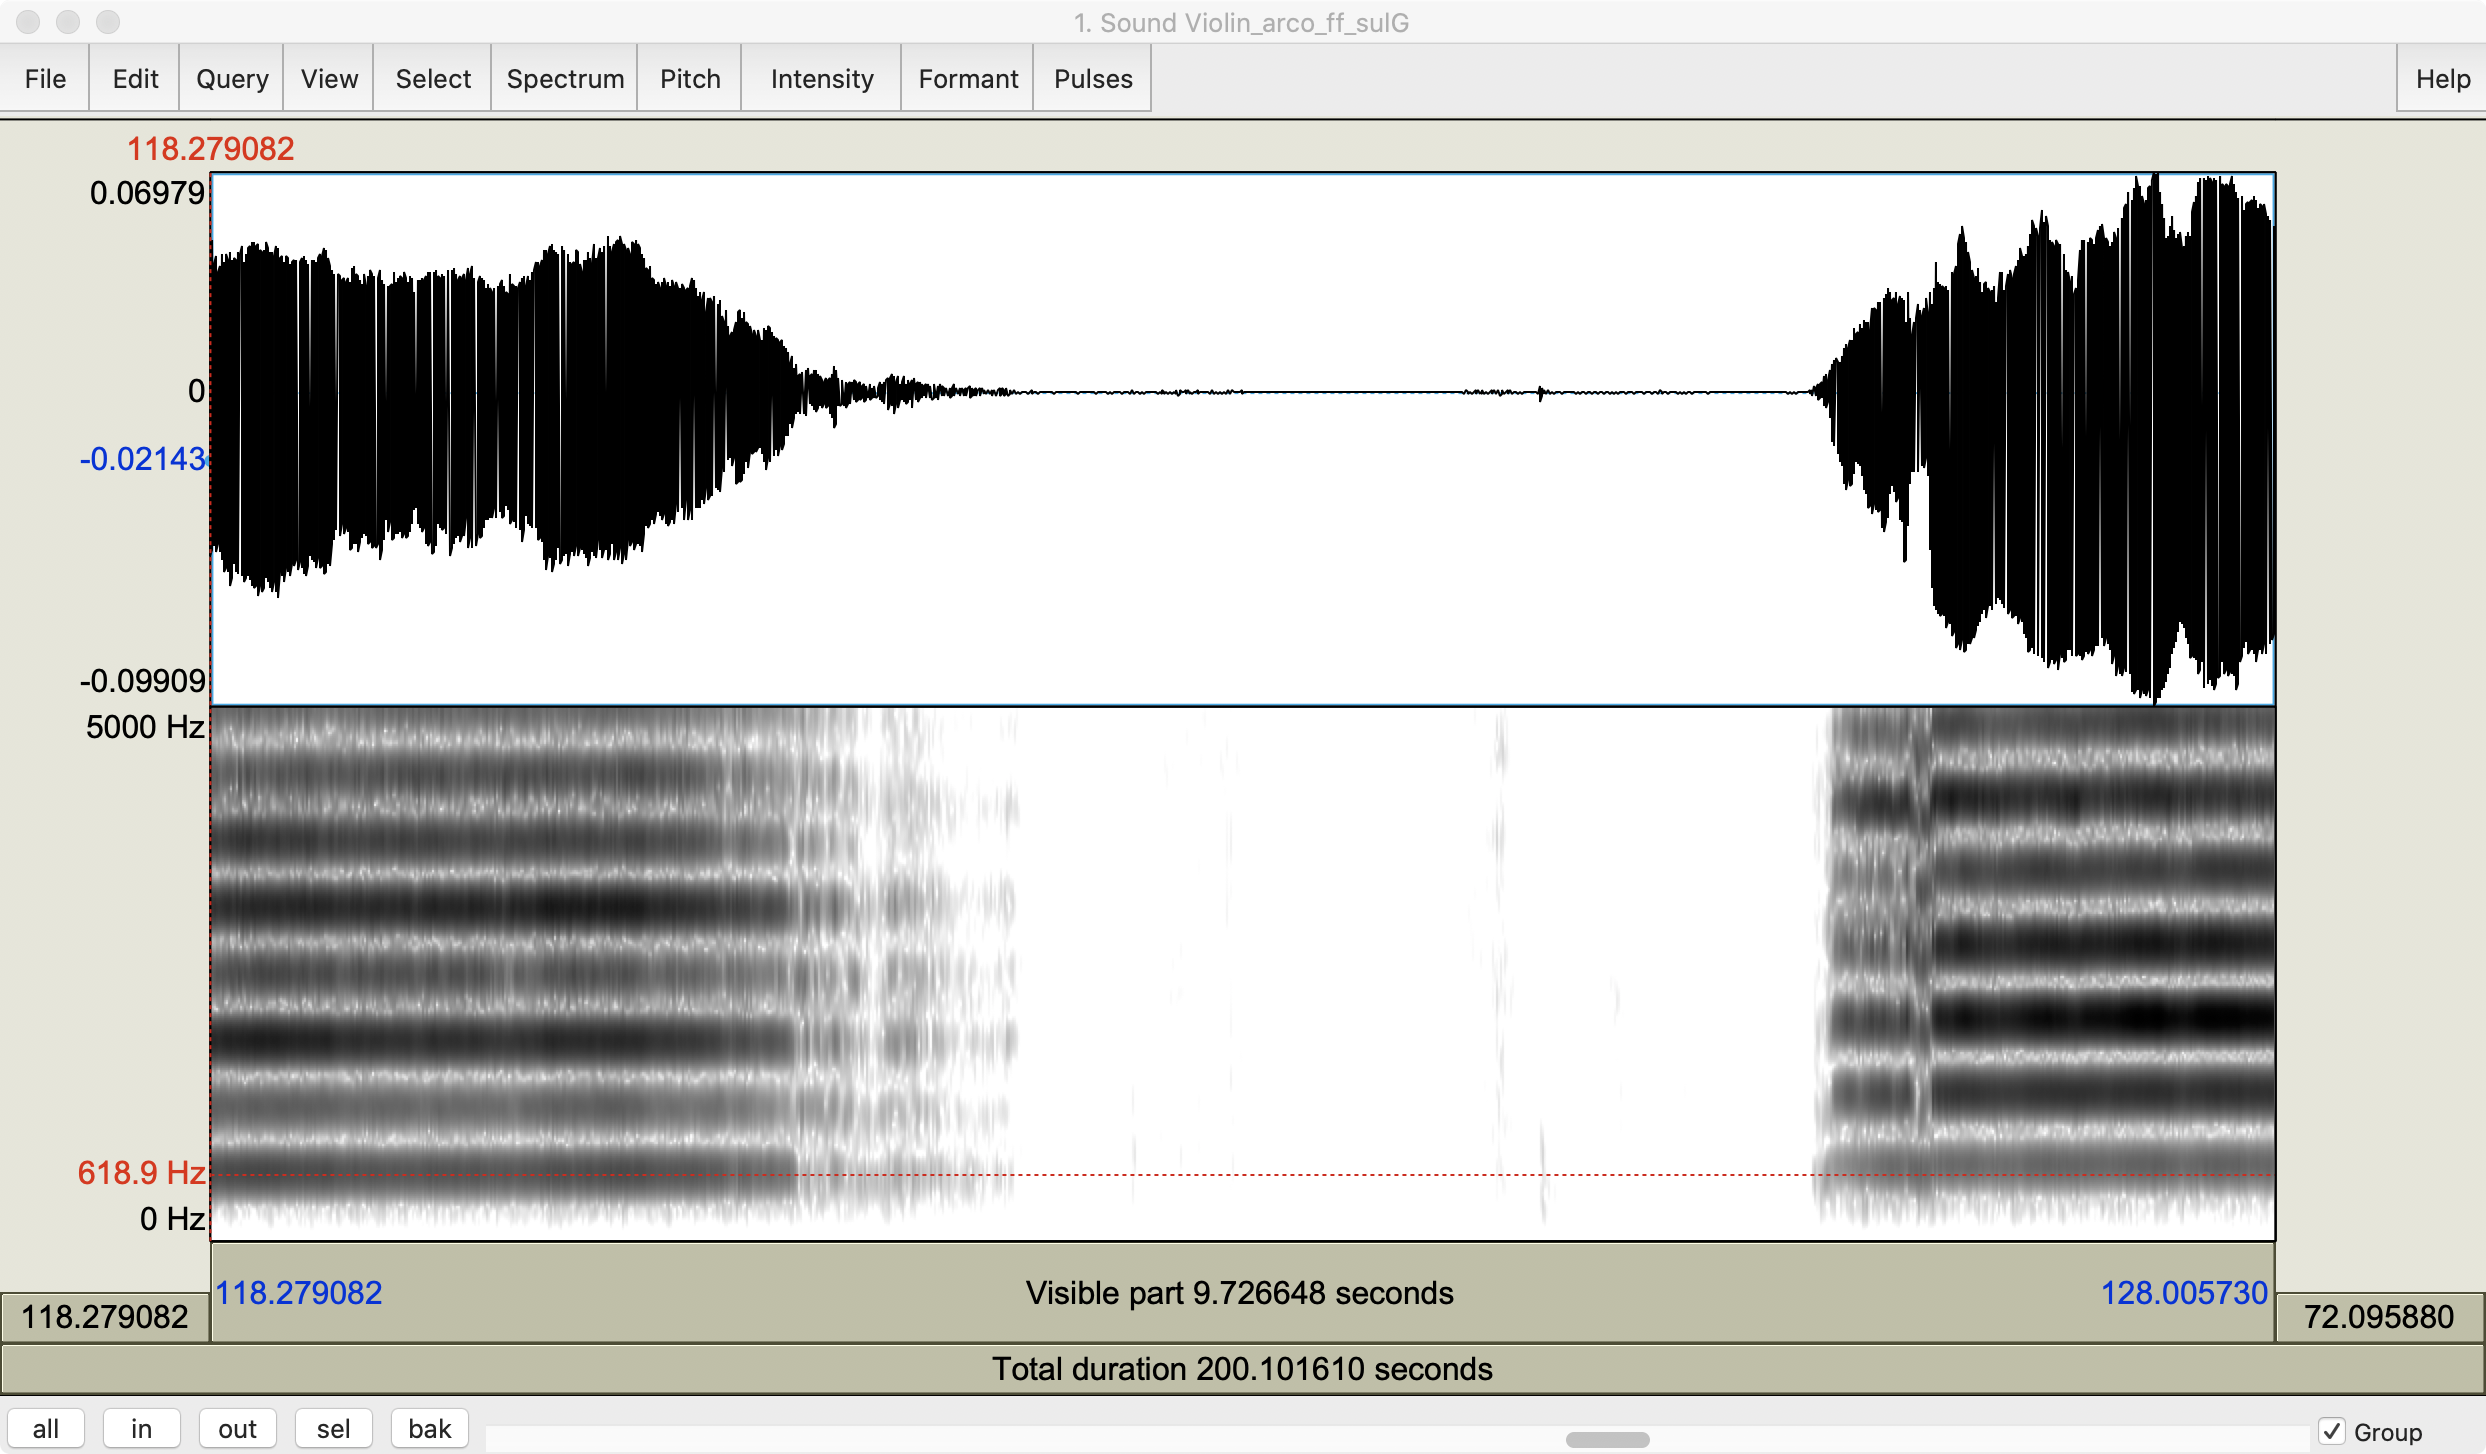
\includegraphics[height=2in]{violin_spectrogram.png}}
\end{frame}

\begin{frame}
  \frametitle{Pitch Tracking: One frame of the input looks like this}

  Shown: $\log |X(f)|$.  What we'll actually use: $|X[k]|$.
  
  \centerline{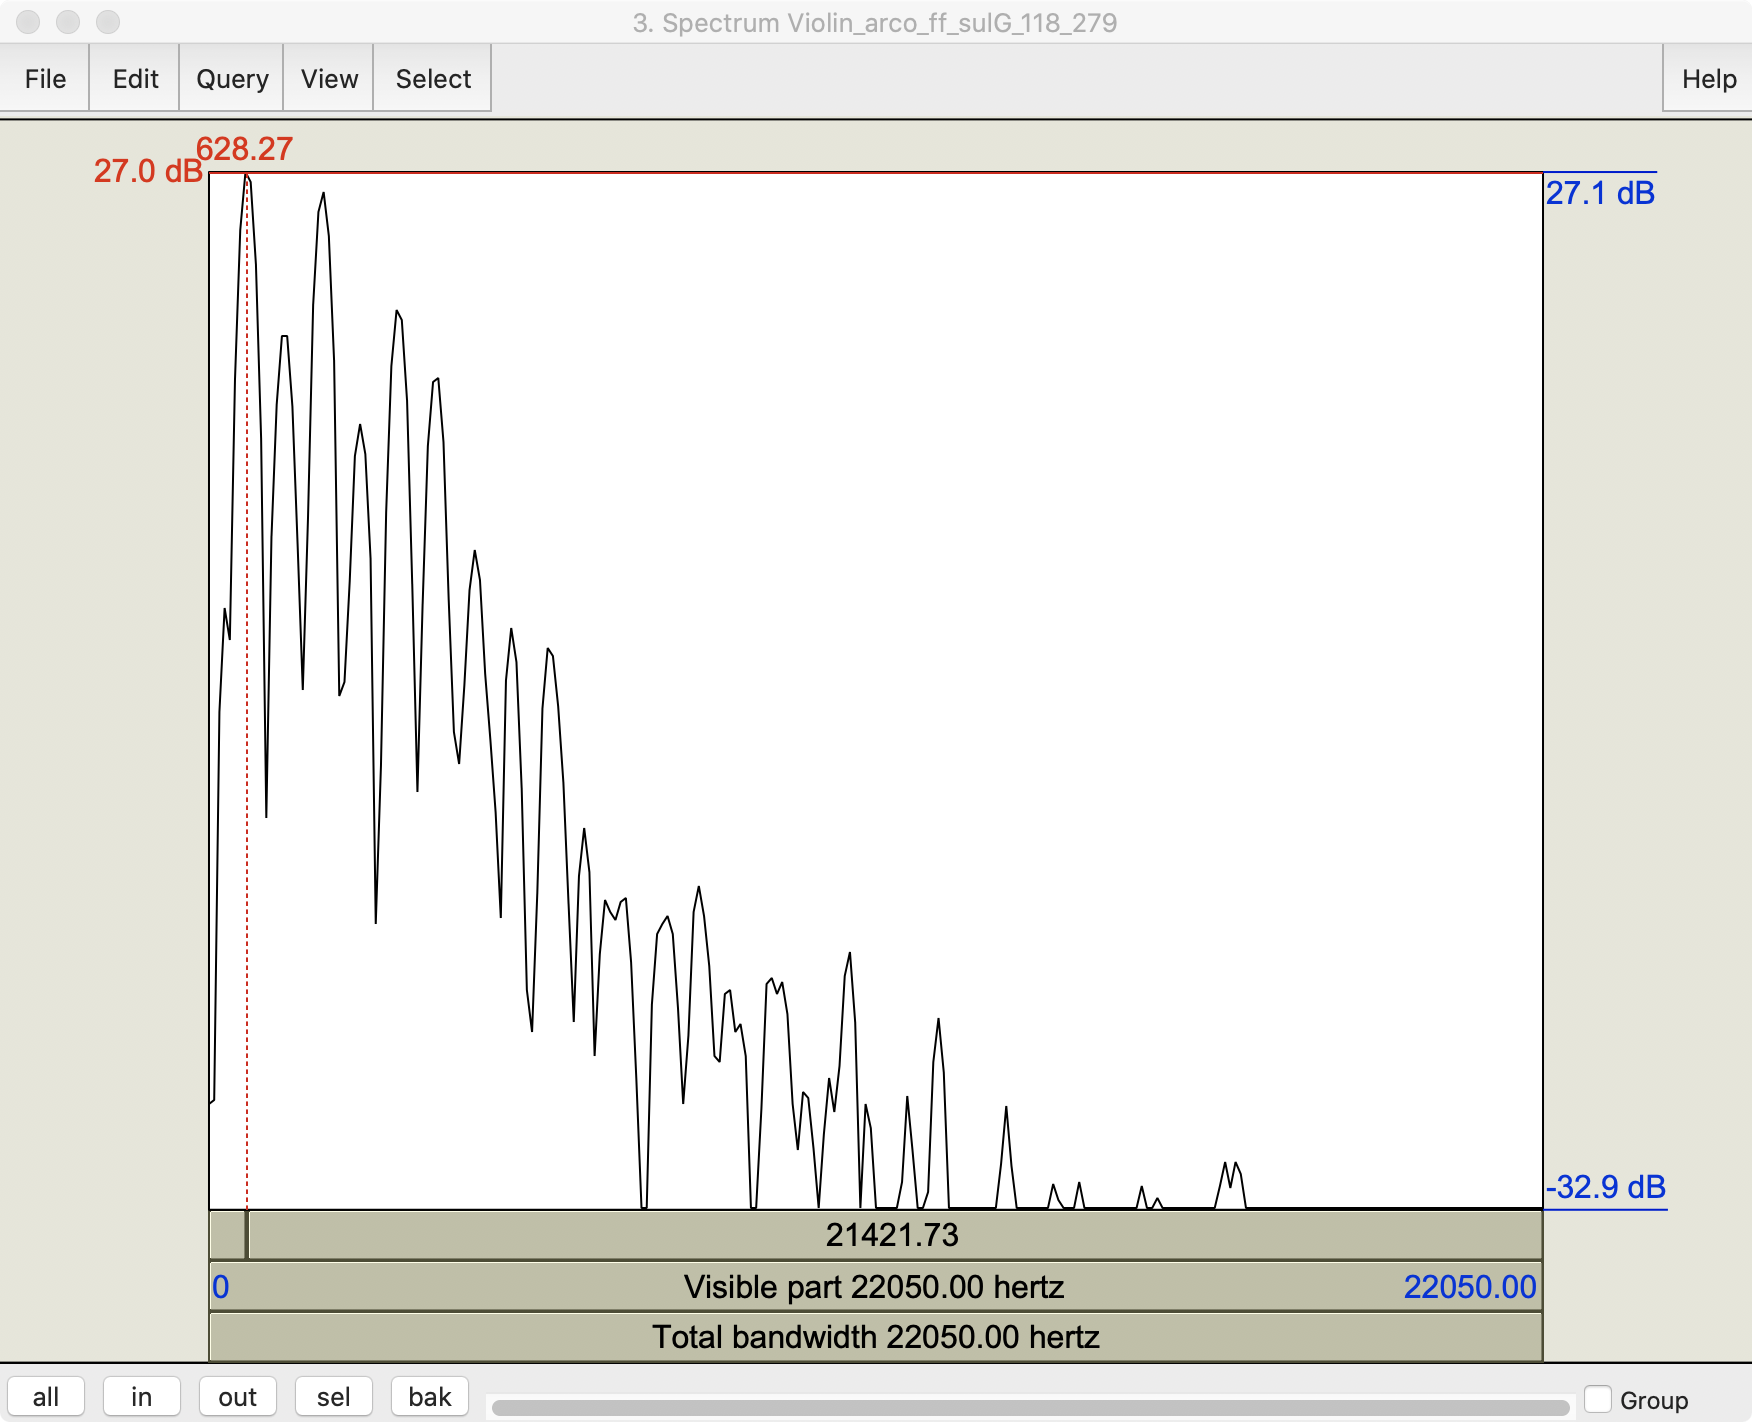
\includegraphics[height=2in]{violin_spectral_slice.png}}
\end{frame}

\begin{frame}
  \frametitle{Pitch Tracking: Input and Output}
  \centerline{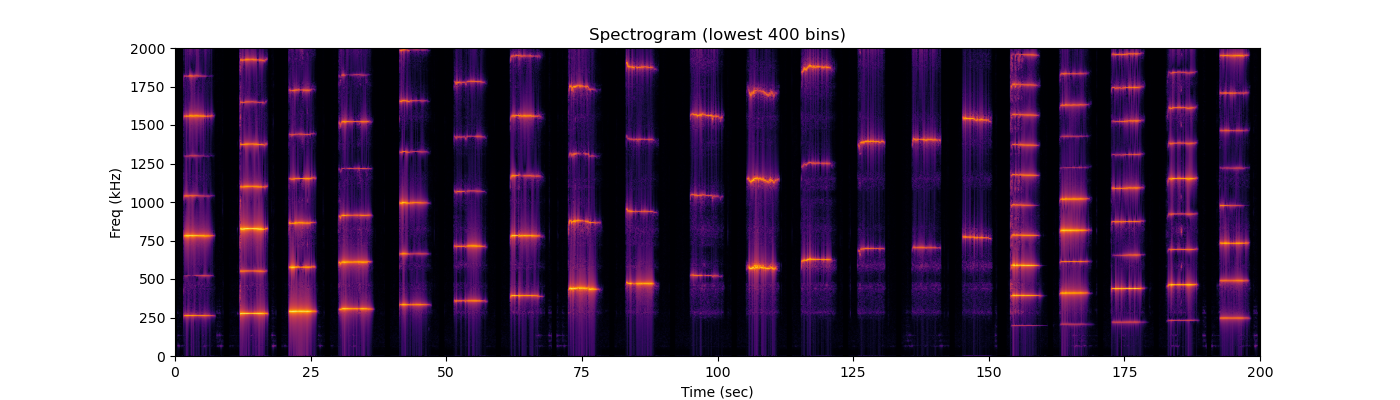
\includegraphics[height=1.5in]{scale_spectrogram.png}}
  \centerline{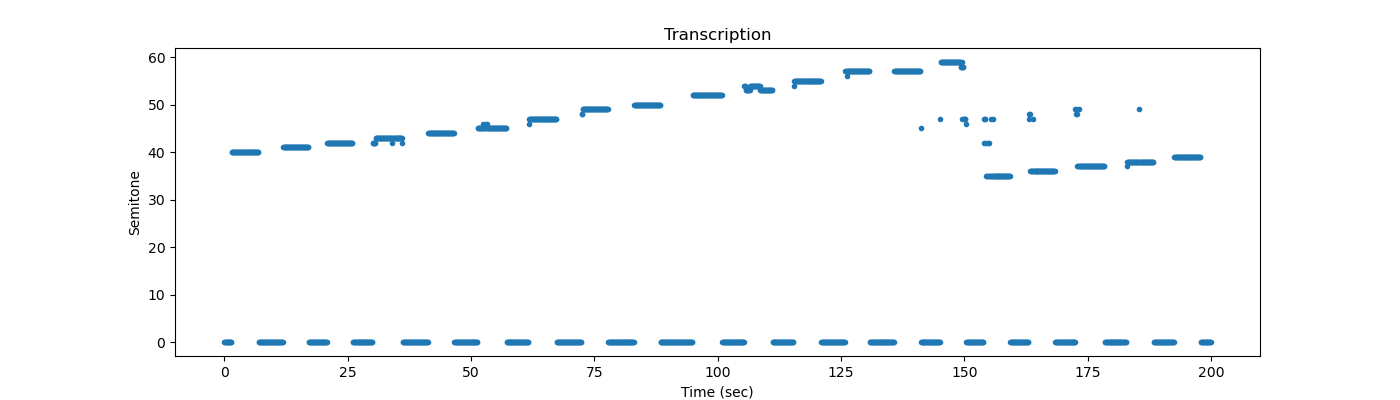
\includegraphics[height=1.5in]{scale_pitches.png}}
\end{frame}

\begin{frame}
  \frametitle{The Harmonic Sieve Algorithm: Overview}
  
  \centerline{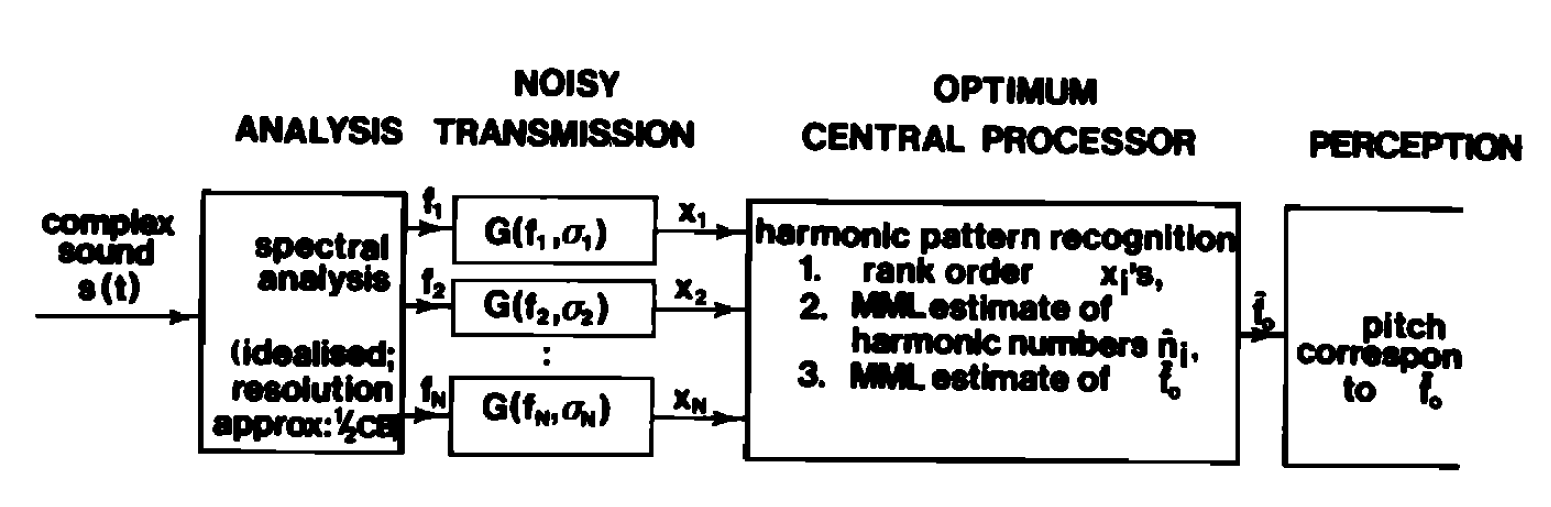
\includegraphics[height=1.5in]{duifhuis1.png}}
  \begin{tiny}
    (c) Duifhuis, Willems \& Sluyter, J. Acoust. Soc. Am. 71(6):1568-1580, 1982
  \end{tiny}
\end{frame}

\begin{frame}
  \frametitle{The Harmonic Sieve}

  \begin{enumerate}
  \item Compute the DFT, $X[k]$.
  \item For any given frequency $f$, define the energy at that
    frequency to include all of the magnitude DFT within $\pm 5$\%, i.e.,
    \[
    E(f) = \sum_{k=0.95(Nf/F_s)}^{(1.05)Nf/F_s} |X[k]|
    \]
  \item In order to test the Goodness of $F_0$ as a possible
    pitch frequency, add up the energy of its first 11 harmonics:
    \[
    G(F_0) = \sum_{h=1}^{11} E(hF_0)
    \]
  \item Choose the pitch with the best goodness.
  \end{enumerate}
\end{frame}

\begin{frame}
  \frametitle{The Harmonic Sieve}

  \begin{itemize}
    \item Notice that the 11 harmonic frequencies are given by:
      \[
      \vec{f}=\left[F_0, 2F_0, 3F_0, \ldots, 11 F_0\right] = F_0 \times\left[1,2,3,\ldots,11\right]
      \] 
    \item Duifhuis, Willems \& Sluyter had the clever idea of
      computing pitch on a semitone scale:
      \[
      S(\vec{f}) = 12\log_2(\vec{f}) = S(F_0) + \vec{M}
      \]
      So you can search all of the 88 keys on a piano by starting with $S=0$ (the lowest note, A0), and
      searching all the way up to S=87 (the highest note, C8).  For each one, you just add
      the harmonic sieve to get the frequencies of all the harmonics:
      \[
      \vec{M} = \left[12\log_2(1), 12\log_2(2), 12\log_2(3),\ldots,12\log_2(11)\right]
      \]
  \end{itemize}
\end{frame}

\begin{frame}
  \frametitle{The Harmonic Sieve}

  \centerline{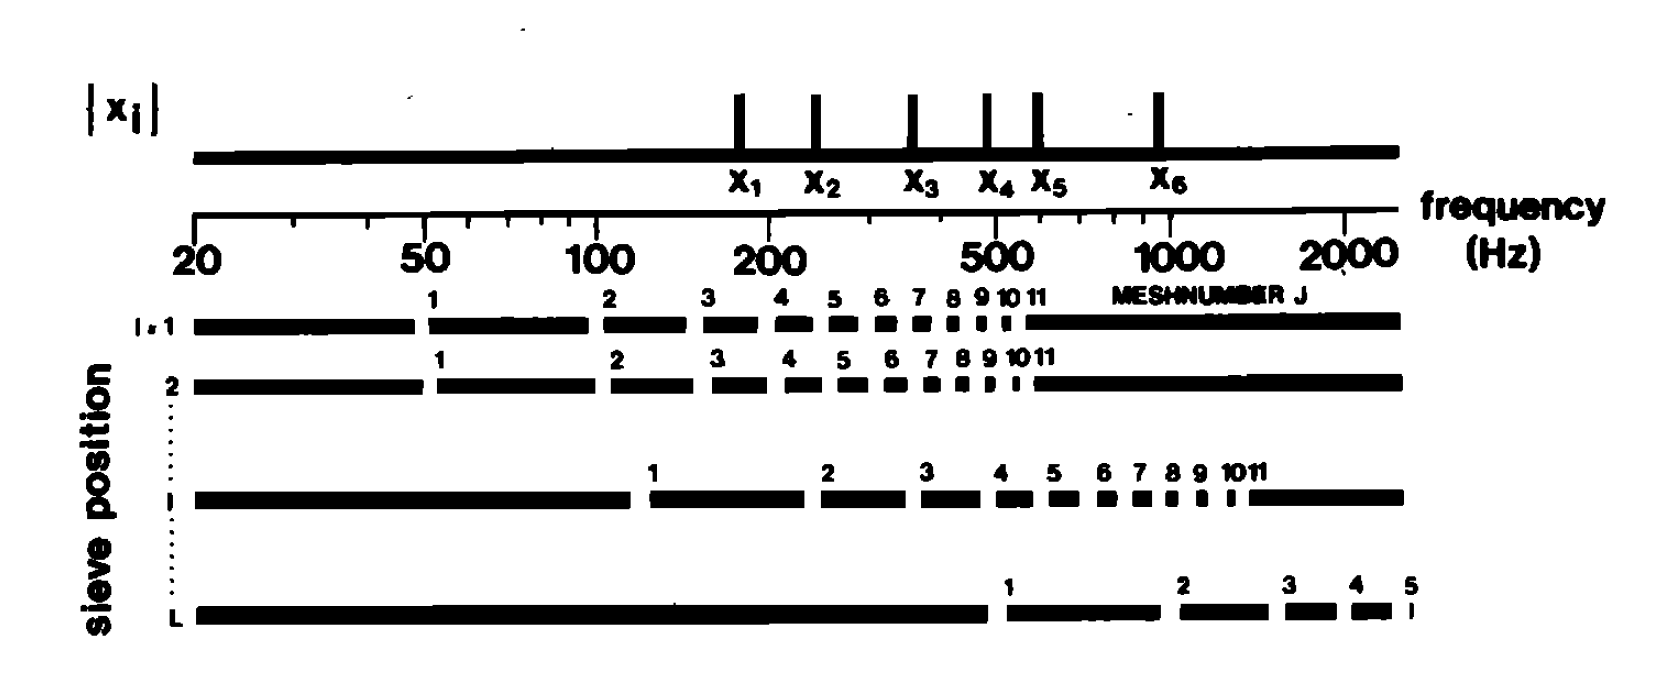
\includegraphics[height=2in]{duifhuis7.png}}
  \begin{tiny}
    (c) Duifhuis, Willems \& Sluyter, J. Acoust. Soc. Am. 71(6):1568-1580, 1982
  \end{tiny}
\end{frame}

\begin{frame}
  \frametitle{Figuring out which bins to average}

  So to figure out which bins to average, for any given pitch $F_0$:
  \begin{enumerate}
  \item Add the pitch in semitones ($S(F_0)$) to the mask ($\vec{M}$).
  \item Convert back into linear frequency:
    \[
    k = \left(\frac{N}{F_s}\right) 2^{(S(F_0)+\vec{M})/12}
    \]
  \end{enumerate}
\end{frame}
    
\begin{frame}
  \frametitle{Masks for each of the notes on the piano}
  \centerline{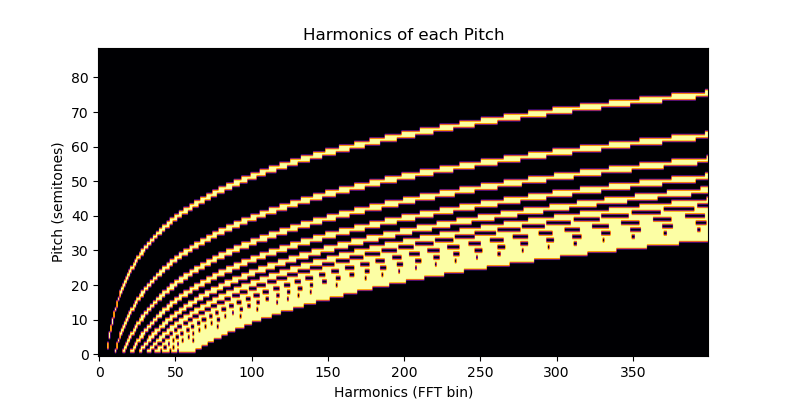
\includegraphics[height=2.5in]{harmonics.png}}
\end{frame}

\begin{frame}
  \frametitle{Duifhuis-Willems-Sluyter Spectral Analysis}

  \begin{itemize}
  \item Duifhuis, Willems \& Sluyter also used a ``peak detector''
    step, after their amplitude spectrum, in order to extract peaks
    from the spectrum before they applied the sieve.
  \item I found this step to be
    unnecessary when I was designing MP2.
  \item On the other hand, this kind of peak detection is used used by
    Shazam, Soundhound, Beatfind, Google Sound Search etc., to reduce
    the number of bits per song, so that they can efficiently identify
    the song you're listening to.  So you might find that part of the
    Duifhuis et al. article interesting, even though we're not using
    it in MP2.
  \end{itemize}
\end{frame}
  
\begin{frame}
  \frametitle{Duifhuis-Willems Spectral Analysis}

  \centerline{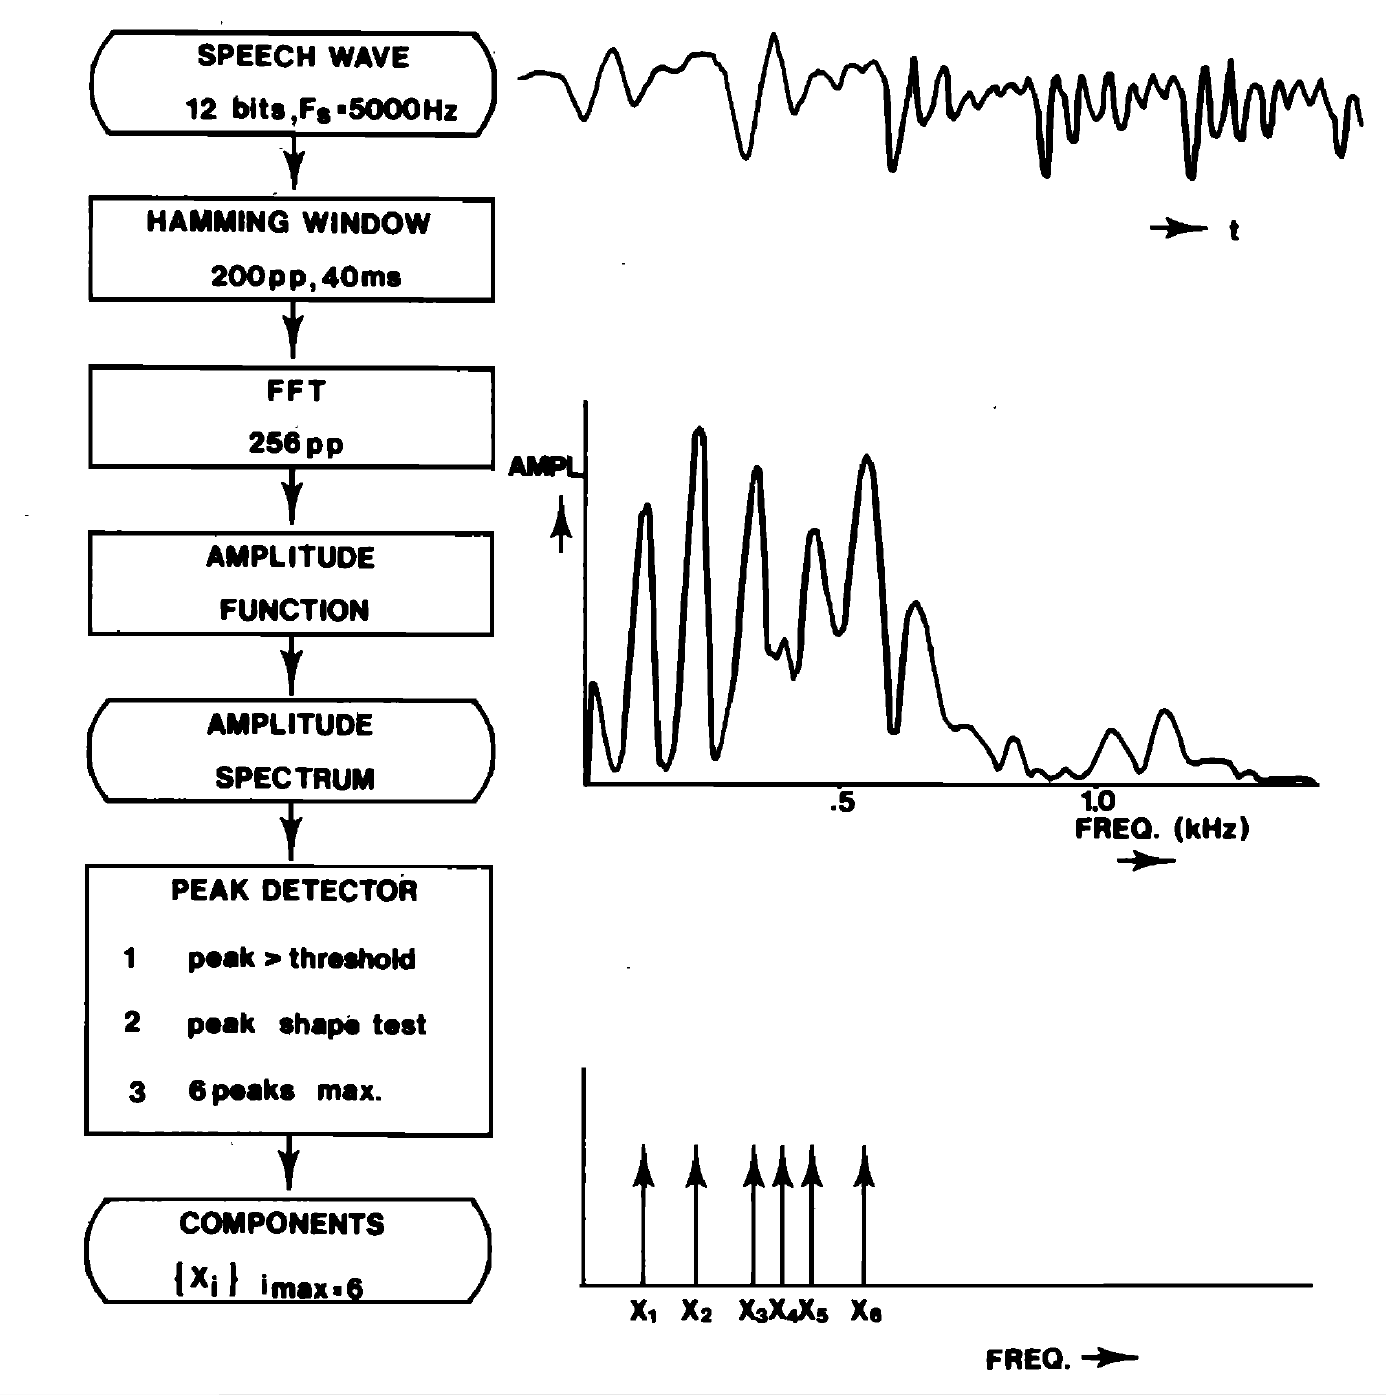
\includegraphics[height=3in]{duifhuis6.png}}
  \begin{tiny}
    (c) Duifhuis, Willems \& Sluyter, J. Acoust. Soc. Am. 71(6):1568-1580, 1982
  \end{tiny}
\end{frame}


%%%%%%%%%%%%%%%%%%%%%%%%%%%%%%%%%%%%%%%%%%%%
\section[Phase Vocoder]{Music Synthesis: the Phase Vocoder}
\setcounter{subsection}{1}

\begin{frame}
  \frametitle{Fourier Synthesis}

  Suppose you know $X[k]$.  How can you get $x[n]$ back again?

  That's right!
  \[
  x[n] = \frac{1}{N}\sum_{k=0}^{N-1} X[k] e^{j2\pi kn/N}
  \]
\end{frame}

\begin{frame}
  \frametitle{Fourier Synthesis without phase}

  Suppose you know the {\bf magnitude only}, $|X[k]|$.  How can you
  get $x[n]$ back again?
  \begin{itemize}
  \item Pretend that $\angle X[k]=0$.  Oops.  Sounds like a click.
  \item Pretend that $\angle X[k]$ is a random number between $0$ and
    $2\pi$.  Oops.  Sounds like noise.
  \item Be smart about the relationship between frequency and phase.
  \end{itemize}
\end{frame}

\begin{frame}
  \frametitle{The relationship between frequency and phase}

  Notice that we could write
  \[
  A\cos\left(2\pi ft+\theta\right)=A\cos(\phi(t))
  \]
  where $\phi(t)$ is the instantaneous phase:
  \begin{itemize}
  \item at time $t=0$, the instantaneous phase is just
    \[
    \phi(0) = \theta
    \]
  \item At the end of a $T$-second frame,
    \[
    \phi(T) = \phi(0)+2\pi fT
    \]
  \end{itemize}
\end{frame}

\begin{frame}
  \frametitle{The phase vocoder}

  At  each time $t$, for each of the DFT frequency bins $k$:
  \begin{enumerate}
  \item Decide whether $|X_t[k]|$ is one of the harmonics of a tone, or just noise.
  \item If it's just noise, set $\phi_k(t)$ to a random number between $0$ and $2\pi$.
  \item If it's a pure tone, set $\phi_k(t)=\phi_k(t-T)+2\pi f_k T$,
    where $f_k$ is the center frequency ($kF_s/N$), and $T$ is the
    length of the frame (in seconds).
  \end{enumerate}
\end{frame}

\begin{frame}
  \frametitle{Result: synthesized magnitudes and phases}
  
  \centerline{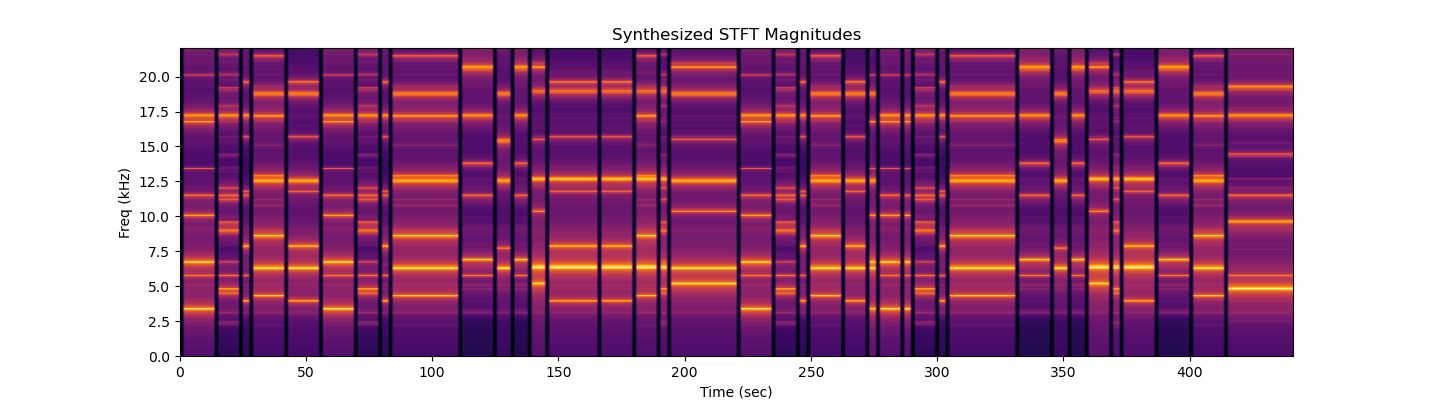
\includegraphics[height=1.5in]{dft_magnitudes.png}}
  \centerline{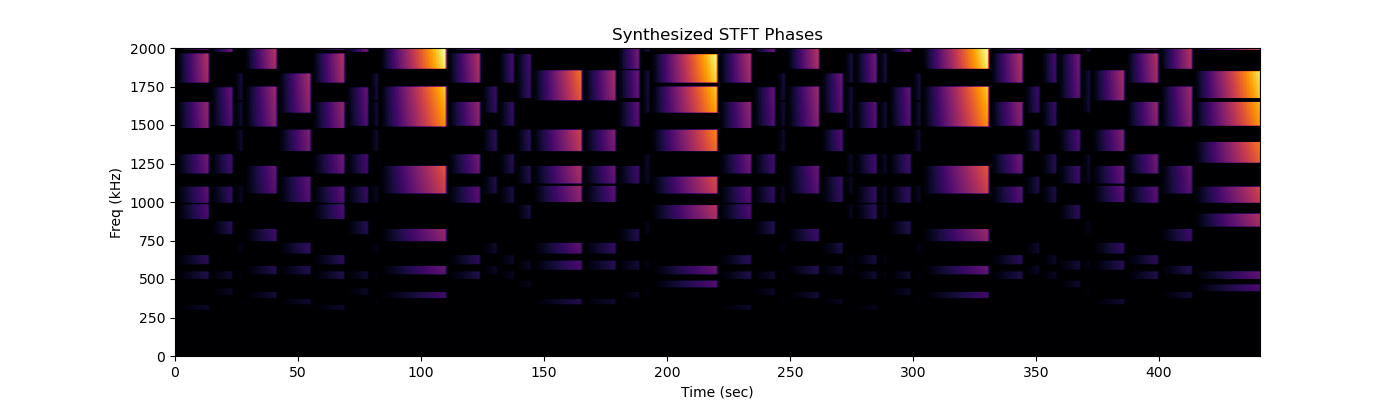
\includegraphics[height=1.5in]{dft_phases.png}}
\end{frame}


%%%%%%%%%%%%%%%%%%%%%%%%%%%%%%%%%%%%%%%%%%%%
\section[Summary]{Summary}
\setcounter{subsection}{1}

\begin{frame}
  \frametitle{Summary}
  \begin{itemize}
  \item {\bf Semitones:} the number of semitones, $s$, separating two
    tones $f_2$ and $f_1$ is given by
    \[
    s = 12\log_2\left(\frac{f_2}{f_1}\right)
    \]
  \item {\bf The Harmonic Sieve algorithm:} choose the pitch with the
    best goodness, defined as
    \[
    G(F_0) = \sum_{h=1}^{11}\sum_{k=0.95(hNF_0/F_s)}^{(1.05)hNF_0/F_s} |X[k]|
    \]
  \item {\bf Phase Vocoder:}
    \begin{itemize}
      \item If $|X[k]|$ is just noise, set $\phi_k(t)$ to a random number between $0$ and $2\pi$.
      \item If $|X[k]|$ is a pure tone, set
        $\phi_k(t)=\phi_k(t-T)+2\pi f_k T$, where $f_k$ is the center
        frequency ($kF_s/N$), and $T$ is the length of the frame (in
        seconds).
    \end{itemize}
  \end{itemize}
\end{frame}  
        
\end{document}
